\chapter{Resultados}

Este trabalho tem como objetivo realizar o controle da posição linear de um carro. Com o sistema de controle agora elaborado, este foi colocado a teste tanto em um ambiente de simulação quanto na bancada, neste capítulo são apresentados os resultados obtidos.

\section{Resultados de simulação}

Seguindo o modelo matemático não linearizado obtido no Capítulo \ref{modelagem}. Foi aplicada uma entrada do tipo degrau como referência, dessa forma, no instante de tempo 1 segundo, aplica-se uma referência constante de posição. As Figuras \ref{fig:simulacao01m} e \ref{fig:simulacao02m} apresentam a resposta para para degraus de referência, respectivamente, de 0,1 m e 0,2 m:

\begin{figure}[H]
    \centering
    \includegraphics[width=0.8\linewidth]{figuras/simulacao_referencia_01m.eps}
    \caption[Simulação do controlador com referência de 0,1 m]{Simulação do controlador com referência de 0,1 m.}
    \label{fig:simulacao01m}
\end{figure}

\begin{figure}[H]
    \centering
    \includegraphics[width=0.8\linewidth]{figuras/simulacao_referencia_02m.eps}
    \caption[Simulação do controlador com referência de 0,2 m]{Simulação do controlador com referência de 0,2 m.}
    \label{fig:simulacao02m}
\end{figure}

Buscando testar o comportamento do controlador para com a alteração da referência, foi aplicado um degrau de referência de 0,1 no instante 1 segundo de tempo e um degrau de referência de 0,2 m no instate 5 segundos. A Figura \ref{fig:simulacao01e02m} mostra o resultado obtido:

\begin{figure}[H]
    \centering
    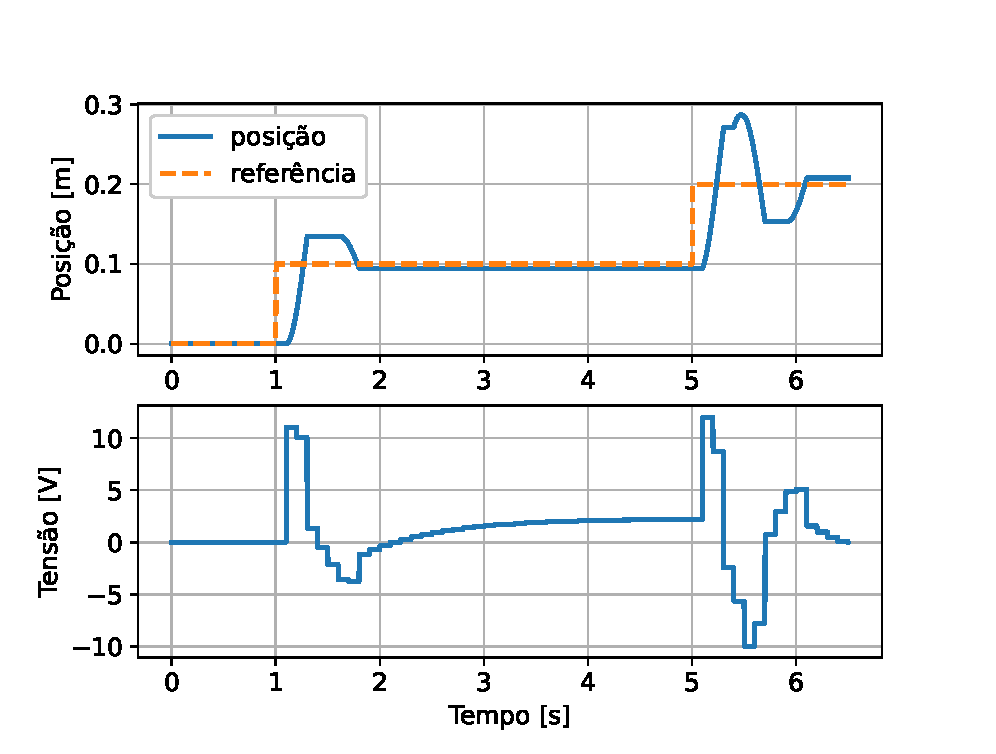
\includegraphics[width=0.8\linewidth]{figuras/simulacao_referencia_01e02m.eps}
    \caption[Simulação do controlador com referência de 0,1 m e 0,2 m]{Simulação do controlador com referência de 0,1 m e 0,2 m.}
    \label{fig:simulacao01e02m}
\end{figure}

Para alcançar o tempo de pico estabelecido como requisito de projeto, a entrada da planta satura temporariamente com a ação de controle, visto que é necessária uma força maior que o atrito seco do carro para começar a movimentar o veículo. Com este em movimento, a ação de controle diminui e não mais satura.

Com os resultados obtidos pode-se observar que existe erro de regime estacionário para referências com menor amplitude, mesmo ainda existindo uma ação de controle. Isso ocorre pois o controlador não considera as limitações físicas da planta, neste caso, a zona morta do motor, que necessita de uma entrada de tensão maior que 3 V para começar a movimentar, impossibilitando o controlador de eliminar o erro de regime estacionário.

Mas para degraus de referência com maior amplitude, a ação de controle para eliminar o erro de regime estacionário não entra na zona morta do motor, permitindo que o carro fique na posição desejada.

Essas mesmas limitações físicas da planta fazem com que o máximo sobressinal seje diferente do requisito de projeto. Como observado, na referência de 0,1 m o máximo sobressinal é menor e na referência de 0,2 m o máximo sobressinal é maior. 

\section{Resultados experimentais}

O mesmo tipo de entrada foi aplicada nos testes na bancada, uma referência do tipo degrau, dessa forma, no instante de tempo 1 segundo, aplica-se uma referência constante de posição. As Figuras \ref{fig:controlador01m} e \ref{fig:controlador02m} apresentam a resposta para para degraus de referência, respectivamente, de 0,1 m e 0,2 m:

\begin{figure}[H]
    \centering
    \includegraphics[width=0.8\linewidth]{figuras/controlador_referencia_01m.eps}
    \caption[Dados experimentais do controlador com referência de 0,1 m]{Dados experimentais do controlador com referência de 0,1 m.}
    \label{fig:controlador01m}
\end{figure}

\begin{figure}[H]
    \centering
    \includegraphics[width=0.8\linewidth]{figuras/controlador_referencia_02m.eps}
    \caption[Dados experimentais do controlador com referência de 0,2 m]{Dados experimentais do controlador com referência de 0,2 m.}
    \label{fig:controlador02m}
\end{figure}

Foi testado o comportamento do controlador para com a alteração da referência, foi aplicado um degrau de referência de 0,1 no instante 1 segundo de tempo e um degrau de referência de 0,2 m no instate 5 segundos. A Figura \ref{fig:controlador01e02m} mostra o resultado obtido:

\begin{figure}[H]
    \centering
    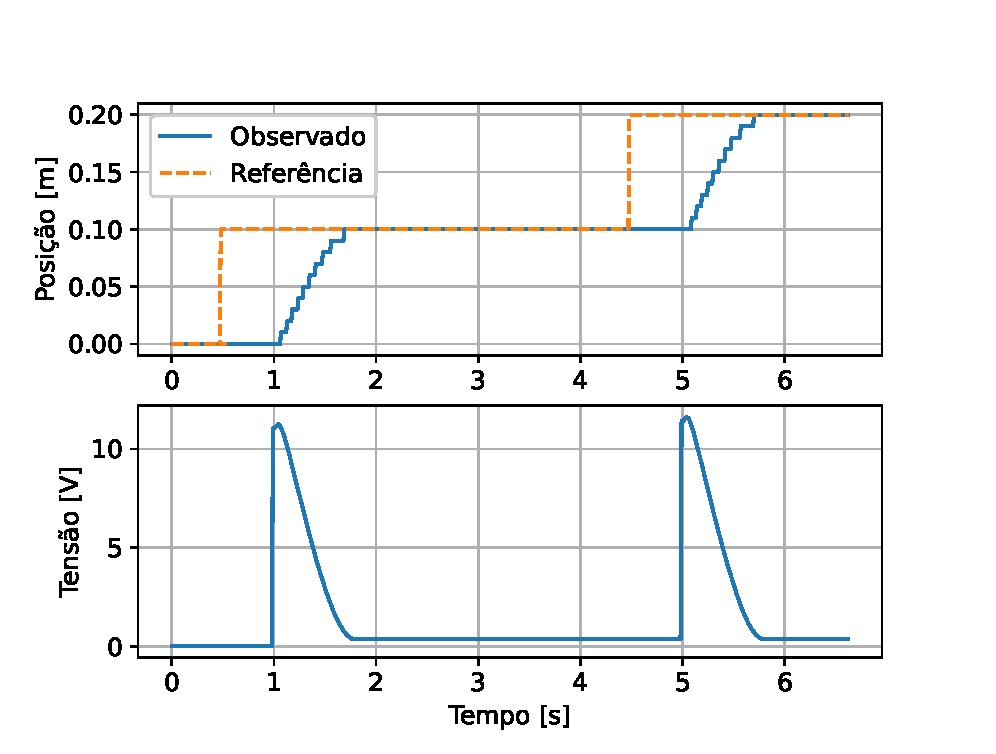
\includegraphics[width=0.8\linewidth]{figuras/controlador_referencia_01e02m.eps}
    \caption[Dados experimentais do controlador com referência de 0,1 m e 0,2 m]{Dados experimentais do controlador com referência de 0,1 m e 0,2 m.}
    \label{fig:controlador01e02m}
\end{figure}

Em todos os casos, a entrada da planta satura no início, ou seja, no momento que é necessário vencer o atrito seco e colocar o carro em movimento, após isso a entrada da planta não satura mais.

Pode ser observado que as limitações físicas da planta tornam o sistema mais lento, fazendo com que o carro para de se movimentar no momento que atinge a sua posição de referência, mesmo que no instante que atinja ainda exista ação de controle. Assim, não existe erro de regime estacionário, mesmo que não ocorra nem máximo sobressinal e nem tempo de pico. 

\section{Comparação entre os Resultados}

Com os resultados obtidos tanto em simulacão quanto os experimentais, foram plotadas as respostas para uma entrada degrau de referência de 0,2 m na seguinte figura:

\begin{figure}[H]
    \centering
    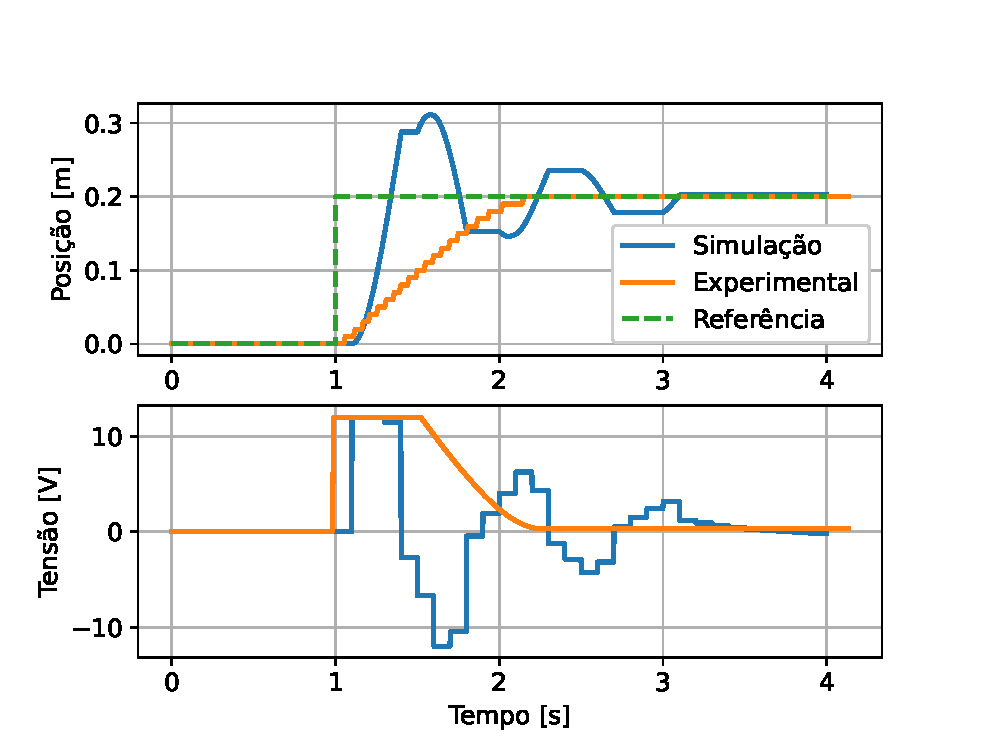
\includegraphics[width=0.8\linewidth]{figuras/controlador_comparacao.eps}
    \caption[Comparação entre os dados experimentais e simulação do controlador com referência de 0,2 m]{Comparação entre os dados experimentais e simulação do controlador com referência de 0,2 m.}
    \label{fig:controlador_comparacao}
\end{figure}

Em ambos os casos as limitações da planta provocam uma diferença com os requisitos de projeto estipulados, entre elas a mais significante é a zona morta do motor. Mesmo assim, tanta na simulação quanto no experimento o controlador atinge a posição desejada e elimina o erro de regime estacionário, embora tenha respostas distintas no regime transiente.